\documentclass[conference]{IEEEtran}
\IEEEoverridecommandlockouts
\usepackage{cite}
\usepackage{amsmath,amssymb,amsfonts}
\usepackage{algorithmic}
\usepackage{graphicx}
\usepackage{textcomp}
\usepackage{xcolor}
%\usepackage{arydshln}

%\usepackage{authblk}
\def\BibTeX{{\rm B\kern-.05em{\sc i\kern-.025em b}\kern-.08em
    T\kern-.1667em\lower.7ex\hbox{E}\kern-.125emX}}
\begin{document}

%\author{
%\IEEEauthorblockN{Wenqing Liu \textsuperscript{*}}
%\and
%\IEEEauthorblockN{Kunli Lin \textsuperscript{*}}
%\and
%\IEEEauthorblockN{Kun Zhang \textsuperscript{*}}
%\and
%\IEEEauthorblockN{Bibo Tu \textsuperscript
%\thanks{Identify applicable funding agency here. If none, delete this.}}
%}
%Kunli Lin,Kun Zhang,Bibo Tu}
\title{HyperMI: A Privilege-level VM Protection Approach against Compromised Hypervisor}
\author{

\IEEEauthorblockN{Wenqing Liu \textsuperscript{},Kunli Lin \textsuperscript{},Kun Zhang \textsuperscript{},Bibo Tu \textsuperscript{*}
\thanks{Bibo Tu is the corresponding author (tubibo@iie.ac.cn).}}%Identify applicable funding agency here. If none, delete this.}}


%\author{\IEEEauthorblockN{Wenqing Liu,Kunli Lin,Kun Zhang,Bibo Tu}
\IEEEauthorblockA{\textit{\textsuperscript{} Institute of Information Engineering, Chinese Academy of Sciences} \\
\textit{\textsuperscript{} School of Cyber Security, University of Chinese Academy of Sciences}\\
%\{xxx\}@iie.ac.cn}%
\{liuwenqing,linkunli,zhangkun,tubibo\}@iie.ac.cn}

}
\maketitle

%\author[a,b]{Wenqing Liu}
%\author[a,b]{Kunli Lin}
%\author[a,b]{Bibo Tu \thanks{Corresponding author: tubibo@iie.ac.cn}}
%\author[a,b]{Kun Zhang}
%\affil[a]{Institute of Information Engineering, Chinese Academy of Sciences}
%\affil[b]{School of Cyber Security, University of Chinese Academy of Sciences}
%\authorcr \{liuwenqing, linkunli, tubibo\}@iie.ac.cn}
%\renewcommand\Authands{ and }

\begin{abstract}
Sensitive data in guest virtual machine is easy to be leaked once hypervisor is compromised.
Therefore, VM protection is important to protect the memory of VM from compromised hypervisor’s malicious access causally. Previous efforts employ hardware or employ new software relying on a higher privilege level than hypervisor.

This paper proposes HyperMI, a novel approach that provides a privilege-level secure execution environment for VM protection in cloud computing against compromised hypervisor. 
It provides HyperMI world, effective VM isolation and event-driven VM monitoring in order to prevent customers' sensitive data in VM from being leaked.
HyperMI world, placed at the same privilege level with hypervisor, is a privilege-level secure isolated execution environment. As TCB, it is used for VM isolation and VM monitoring. 
What's the most important, HyperMI focuses on decoupling the function of interaction between hypervisor and VM and decoupling the function of address mapping of VM from hypervisor.
As a result, HyperMI can only controls page mapping of VM and EPT updating when a page is allocated to a VM.
We have implemented a prototype for KVM hypervisor with multiple Linux as guest OSes, which can be used in commercial
cloud computing industry with portability and compatibility for all kinds of CPU platforms. The security analysis shows that this approach can provide protection for VM with effective isolation and event-driven monitoring, and the performance evaluation confirms the efficiency of HyperMI.



%Remote or local adversaries can easily access other customers' sensitive data in the memory or subvert other guest virtual machines (VMs), once the hypervisor is compromised and controlled by them. 
%Therefore, it is essential to protect VMs, especially the context and the memory of VMs, against the compromised hypervisor.
%%Some previous efforts depend on a higher prigilege level which require large-scale modifications to current commercial cloud software stacks. The other efforts require the addition of extra customized hardware or new hardware with new hardware capabilities, which undoubtedly increase the cost of cloud service providers. 	
%%However, previous efforts employ extra customized hardware which is not convenient for cloud providers to adopt widely. Or they employ new software relying on a higher privilege level than hypervisor. 
%Some previous efforts rely on extra customized hardware and higher privileged system components.
%These approaches increase both the maintenance effort and the code base size of privileged system components, which consequently increases the risk of having security vulnerabilities.
%
%This paper proposes HyperMI, a privilege-level VM protection approach against the compromised hypervisor. 
%% a novel approach to provide runtime protection for VMs based on a privilege-level secure execution environment against compromised hypervisor. 
%%We create HyperMI World as a trusted execution environment witch is isolated from the compromised hypervisor. 
%HyperMI is designed to be placed at the same privilege-level with the compromised hypervisor, it is smoothly embedded into the current commercial cloud environment, which presents no requirements for the upper VMs and the underlying existing hardware. HyperMI can be applied to multi-platforms too. 
%% and can be applied to multi-platforms. HyperMI also does not change the architecture of 
%%and does not rely on any additional hardware or a higher privileged level than the hypervisor. 
%%Firstly, HyperMI can intercept interaction data between all VMs and hypervisor and redirects interaction process to HyperMI. Secondly, HyperMI achieves effective VM memory isolation to provide runtime protection for VMs by page marking technology.
%%isolating memory among VMs and hypervisor securely. 
%The key of HyperPS is that it decouples the functions of interaction between VM and the hypervisor. As a result, HyperPS monitors the interaction, controls memory mapping when a page is allocated, and resists system information leakage attack.
%We have implemented a prototype for KVM hypervisor on x86 platform with multiple VMs running Linux. KVM with HyperPS can be applied to current commercial cloud computing industry with portability. The security analysis shows that this approach can provide effective monitoring against compromised attack, and the performance evaluation confirms the efficiency of HyperPS.

\end{abstract}

\begin{IEEEkeywords}
Virtualization, VM Protection, VM Security
\end{IEEEkeywords}

\section{Introduction}



\iffalse
As more and more functionalities are added into the hypervisor, the code bases of commodity hypervisors (KVM or Xen) have been increased to be large lines. However, a recent survey shows that commodity hypervisor incurs more vulnerabilities because of the larger code bases. 
On the one hand, from 2004 to now, there are 130 vulnerabilities about KVM.
Some of them (e.g., CVE-2018-1087)
shows high-risk vulnerabilities that can lead to privilege raising behavior and comprehensive compromised hypervisor.
On the other hand, because hypervisor possesses the highest privilege in the cloud environment, an attacker who compromises hypervisor could harm the whole cloud infrastructure and endanger data and computation in the cloud. For example, an attacker can deploy a complete malicious guest VM on the virtualized platform, conducts attacks to the hypervisor and further attack other VMs even the entire platform through illegal data accessing and so on. Some attacks also directly compromise hypervisor.
In order to settle down all these threats, some try to detect malicious actions among frequent cloud management operations, but this kind of approach is much similar to that of looking for a needle in a haystack. Therefore, HyperMI could provide a superior solution from another perspective. 
Current researches
%, including customized hardware, reconstructed hypervisor, and software placed at a higher privilege-level than the hypervisor, 
provide services of protection for critical data.
\fi
As more and more functionalities are added into the hypervisor, the code bases of commodity hypervisors (KVM or Xen) increase to be large lines. On the one hand, commodity hypervisor has more vulnerabilities because of the larger code bases. On the other hand, because the hypervisor possesses the highest privilege in the cloud environment, an attacker who compromises hypervisor can harm the whole cloud infrastructure and endanger data in the cloud.
%In order to protect VM, HyperMI provides a superior solution rather than malicious actions detection.
%Current researches provide services of protection for critical data.
Being aware of such serious situation, current researchers try to alleviate those vulnerabilities by hardware or software on a higher level than the hypervisor.

\textbf{Hardware}
%Some efforts (SecureME\cite{Chhabra2011SecureME}, Bastion\cite{Champagne2010Scalable} and Iso-x\cite{Evtyushkin2015Iso}) rely on 
%customized underlying hardware to provide fine-grained protection for VM or in-VM process. 
%Iso-X provides isolation for security-critical pieces of an application by introducing additional hardware and changes to OS. It controls memory access by introducing ISA instructions. 
%Bastion uses modified microprocessor hardware based on FPGA to protect the storage and runtime memory state of enhanced hypervisor against both software and hardware attacks. So that it provides hardware-protected environment and protection for security-critical OS and application modules in an untrusted software stack. 
Different hardware platforms provide different hardware mechanisms,such as Intel's Software Guard Extensions (SGX) and AMD's Secure Memory Encryption (SME)\cite{WuLLCZG18}.
SGX provides protection for pieces of application logic inside encrypted enclave memory against malicious OS. However, it is limited to protect a relatively small portion
of memory, and the developers have to mostly reconstruct the protected software or build it from scratch. Therefore it is nontrivial for SGX to protect large-scale software like the entire VM. 
SME can encrypt memory in page level granularity by simply setting the C-bit
in the page table entry. More importantly, AMD enables the Secure Encrypted Virtualization (SEV) feature. However, a malicious hypervisor can bypass the protection by manipulating some critical resources, guest memory mapping and key sharing mechanisms.


\iffalse
\textbf{Reconstructed Hypervisor }
Some efforts (NoHype\cite{NoHype} and TrustOSV\cite{TrustOSV}) pre-allocate fixed cores or memory resource to isolate VMs via reconstructing hypervisor. In the meantime, these efforts deprive some virtualization capabilities and introduce lots of modification of the hypervisor. Moreover, NoHype removes the virtualization layer while retaining the key features enabled by virtualization. TrustOSV protects cloud environment by removing interactions between exposed executing environment and hypervisor.
\fi
 
\textbf{Software at Higher Privilege Level}
In order to mitigate the hazard caused by the hypervisor, plenty of software solutions propose and introduce a higher privilege-level than the original hypervisor. Nested virtualization is one of the representative approaches, which provides a higher-privileged and isolated execution environment to run the monitor securely. The turtles project \cite{Ben2007The} and CloudVisor \cite{Zhang2011CloudVisor} are examples of systems that propose nested virtualization idea to achieve isolation for protected resources. Especially, CloudVisor uses nested virtualization to decouple resource management into the nested hypervisor to protect VMs. %It is no doubt that these approaches 
%based on a higher privilege level than hypervisor would
 %introduce lots of inter-privilege-level transition and larger code base.

\iffalse
In practice, independence on platforms is among the most prized features for cloud providers. Furthermore, business architectures that are already widely deployed, it is equally important to minimize changes to existing systems. For this purpose,
some recent efforts only focus on software approaches about how to achieve the same privilege-level isolation and protection without relying on a higher privilege level. For example, SKEE\cite{Azab2016SKEE} introduces a secure execution environment at the same privilege level with kernel. A hardware approach on Intel, SGX, provides protection for applications but VMs. It also needs a lot of programming for every application.
\fi

In practice, the independence on platforms and minimum changes to existing systems are the most prized features for cloud providers. For this purpose,
some recent efforts introduce software-based approaches that achieve the same privilege-level isolation and protection instead of relying on a higher privilege level. 
%For example, SKEE\cite{Azab2016SKEE} introduces a secure execution environment at the same privilege level with kernel.
% Intel's SGX, a hardware approach, is designed to provide protection for applications instead of the whole VM.  SGX can isolate critical applications from the cloud platform it runs (the VMM, the VMs and firmware). 
% however this feature is only available in the newly released hardware. 
  %It also needs a lot of programming for every application.



Inspired by the idea of "same privilege-level" isolation, we propose HyperMI, a "same privilege-level" and software-based VM protection approach for guest VMs against the compromised hypervisor. 
%HyperMI introduces a secure isolation execution environment, named HyperMI World, to place runtime data and VM memory isolation module. 
With HyperMI, interaction data protection and VM memory isolation modules are resided in a secure execution environment, referred to as HyperMI World.
%The VM monitoring module provides monitoring for the interaction between the compromised hypervisor and each VM. 
%The VM isolation module guarantees memory isolation between VMs. 
%The details on them are as follows with taking x86 platform as an example.
We implement this prototype on x86 as an example, more details on HyperMI are described as follows.

%\textbf{VM Protection}
%这部分是介绍,所以不需要详细讲,只需要讲清楚为什么要保护这些数据,具体怎么保护这些数据,怎么hook到安全空间是在设计的部分时候讲。
%为什么要保护这些数据,首先要明确恶意的hypervisor威胁上面的虚拟机存在两种方式,修改虚拟机上下文信息或者修改虚拟机运行内容,因此这两部分内容需要额外保护起来。然后再讲保护这部分东西是通过事件驱动的方式,而非周期,具体如何事件驱动的时候,只需要写相应的写操作的时候,decouple到hyperMI中,具体如何保护,由设计部分讲,一句话说明。
HyperMI protects interactions between hypervisor and VM and achieves memory isolation among VMs. 
%Thus, the compromised hypervisor could not subvert the domain of the state of VMs. 
There are some especially critical interaction structures data that records state information of VMs HyperMI should protect. These data includes Extended Page Tables (EPT) and Virtual Machine Control Structure (VMCS). EPT contains the mapping relationship from Guest Physical Address (GPA) to Host Physical Address (HPA). 
%the compromised hypervisor can modify the content of any EPT entry, thus maps GPA of VM to an illegal HPA. EPTP is a CR3-like register used to supply CPU with the address of EPT, thus the adversary could subvert a VM by supplying CPU with a carefully constructed and illegal EPT. 
VMCS is used in VMX operation to manage the behavior of VMs as well as transitions between the VM and the hypervisor. Thus, the modification of context of VMCS, especially the Guest-state area and VM-execution control fields, may cause unpredictable consequences. %poses an uncontrollable impact on the security of VM. 
%Based on the importance of the data structures mentioned above, HyperMI must protect them. 
%Secondly, HyperMI adopts an event-driven monitor approach which hooks events that is closely related to VM exit and VM entry. Once these events occur, monitoring is executed. 
Given the great importance of the data structures mentioned above, HyperMI isolates them beyond access from compromised hypervisor.

%\textbf{VM Isolation}
VM memory isolation can resist malicious VM memory accessing from compromised hypervisor, especially, remapping and double mapping attack.
Firstly, HyperMI marks each page with page marking technique to guarantee each page can only be owned by one VM or hypervisor.
Secondly, it deprives address translation function of the hypervisor to ensure that the page is marked with the owner when it is mapped. 
Finally, since any update to guest page table can be synced to EPT, HyperMI verifies whether any protected virtual addresses is double mapped or remapped.
In order to avoid double mapping attack, the owner of the page is verified when EPT updates.
% to ensure whether access or not when EPT updates resulting from page fault. 
In order to resist remapping attack, HyperMI clears the content of the page when it is released.


Our prototype introduces 4K SLOC (Source Lines of Code) to VM protection and 300 SLOC modifications of the hypervisor.
% VM monitoring reduces the attack surface of the hypervisor, and the memory isolation among hypervisor and VMs is significantly guaranteed. 
The experimental results show trivial performance overhead and independence on multi-platforms for runtime VM protection. 


Our contributions are as follows:
\begin{itemize}
%\item A secure isolated execution environment placed at the same privilege level with hypervisor instead of relying on a higher privilege-level or customized hardware.
%\item{A non-bypassable hypervisor protection for VMCS and EPT approach  which can ensure the security of interactions between hypervisor and VMs.}
\item A secure isolated execution environment placed at the same privilege level with hypervisor instead of relying on a higher privilege-level or hardware.
\item{An approach of isolating memory among VMs and hypervisor securely for VM by using page marking technique to avoid malicious access from compromised hypervisor.}

\item{An unbypassable hypervisor monitoring for VMCS and EPT approach  which can ensure the security of interaction between hypervisor and VM.}

\item{A prototype based on KVM and x86 architecture with trivial performance overhead, high security and portability.}

\end{itemize}
The rest of this paper is organized as follows. Section \ref{sec:threat} discusses our threat model and assumption. Section \ref{sec:design} elaborates on the design and implementation of HyperMI on x86 platform. Section \ref{sec:evaluation} gives the evaluation of security and performance. Section \ref{sec:related} compares HyperMI with previous work. At last, Section \ref{sec:conclusion} gives the conclusion.
 

% 背景


\section{Threat Model and Assumption}\label{sec:threat}


\subsection{Threat Model} \label {threat}


%On the one hand, the attacker can modify the critical interaction data in the context switching process between VMs and hypervisor. On the other hand, the attacker can modify the address mapping of EPT, causing remapping attack and double mapping attack.

We assume that the hypervisor has been compromised and controlled by the powerful adversary. The adversary can implement attacks based on two attack paths. 
First, the adversary can subvert the critical interaction data during the context switching process between VM and the hypervisor. Second, the adversary can tamper values of EPT entry. This can result in remapping attack and double mapping attack.

\paragraph{Modifying the Interaction Data}
For the modification of the critical interaction data during the context switching process, the attacker can obtain the address of VMCS
and modify it, such as HOST\_RIP, GUEST\_CR0, EPTP, et al. For example,
modifying the value of privilege register, CR0, can close DEP mechanism, and modifying CR4 can close SMEP mechanism.

\paragraph{Modifying the Address Mapping of EPT}
Modification of EPT can result in memory information leakage. There are two attack scenes, double mapping, and remapping attack.

\textbf{Scene 1.} 
    For double mapping attack, attackers control and compromise a VM, then obtain the privilege of hypervisor through VM escape attack, and maliciously access the VMCS structure to obtain the value of EPT\_Pointer(EPTP). The attack process is as shown in Figure \ref{fig0}. There are two guest VMs, VM1 (attacker) and VM2 (victim). In this way, EPTP of VM1 and EPTP of VM2 are respectively obtained by attackers. Also, for a guest virtual address (GVA) in VM2, named 'A', is mapped to the corresponding real physical address, named 'B'. For VM1, the real physical address corresponding to the guest virtual address 'C' is 'D', then 'D' is modified to be 'B' by modifying the value of the last page item of EPT. At last, 'A' and 'C' are mapped to the real physical address 'B', no address is mapped to 'D'. Then VM1 can access the data of VM2 successfully through accessing 'B', this attack process is called double mapping attack.

\begin{figure}
\centerline{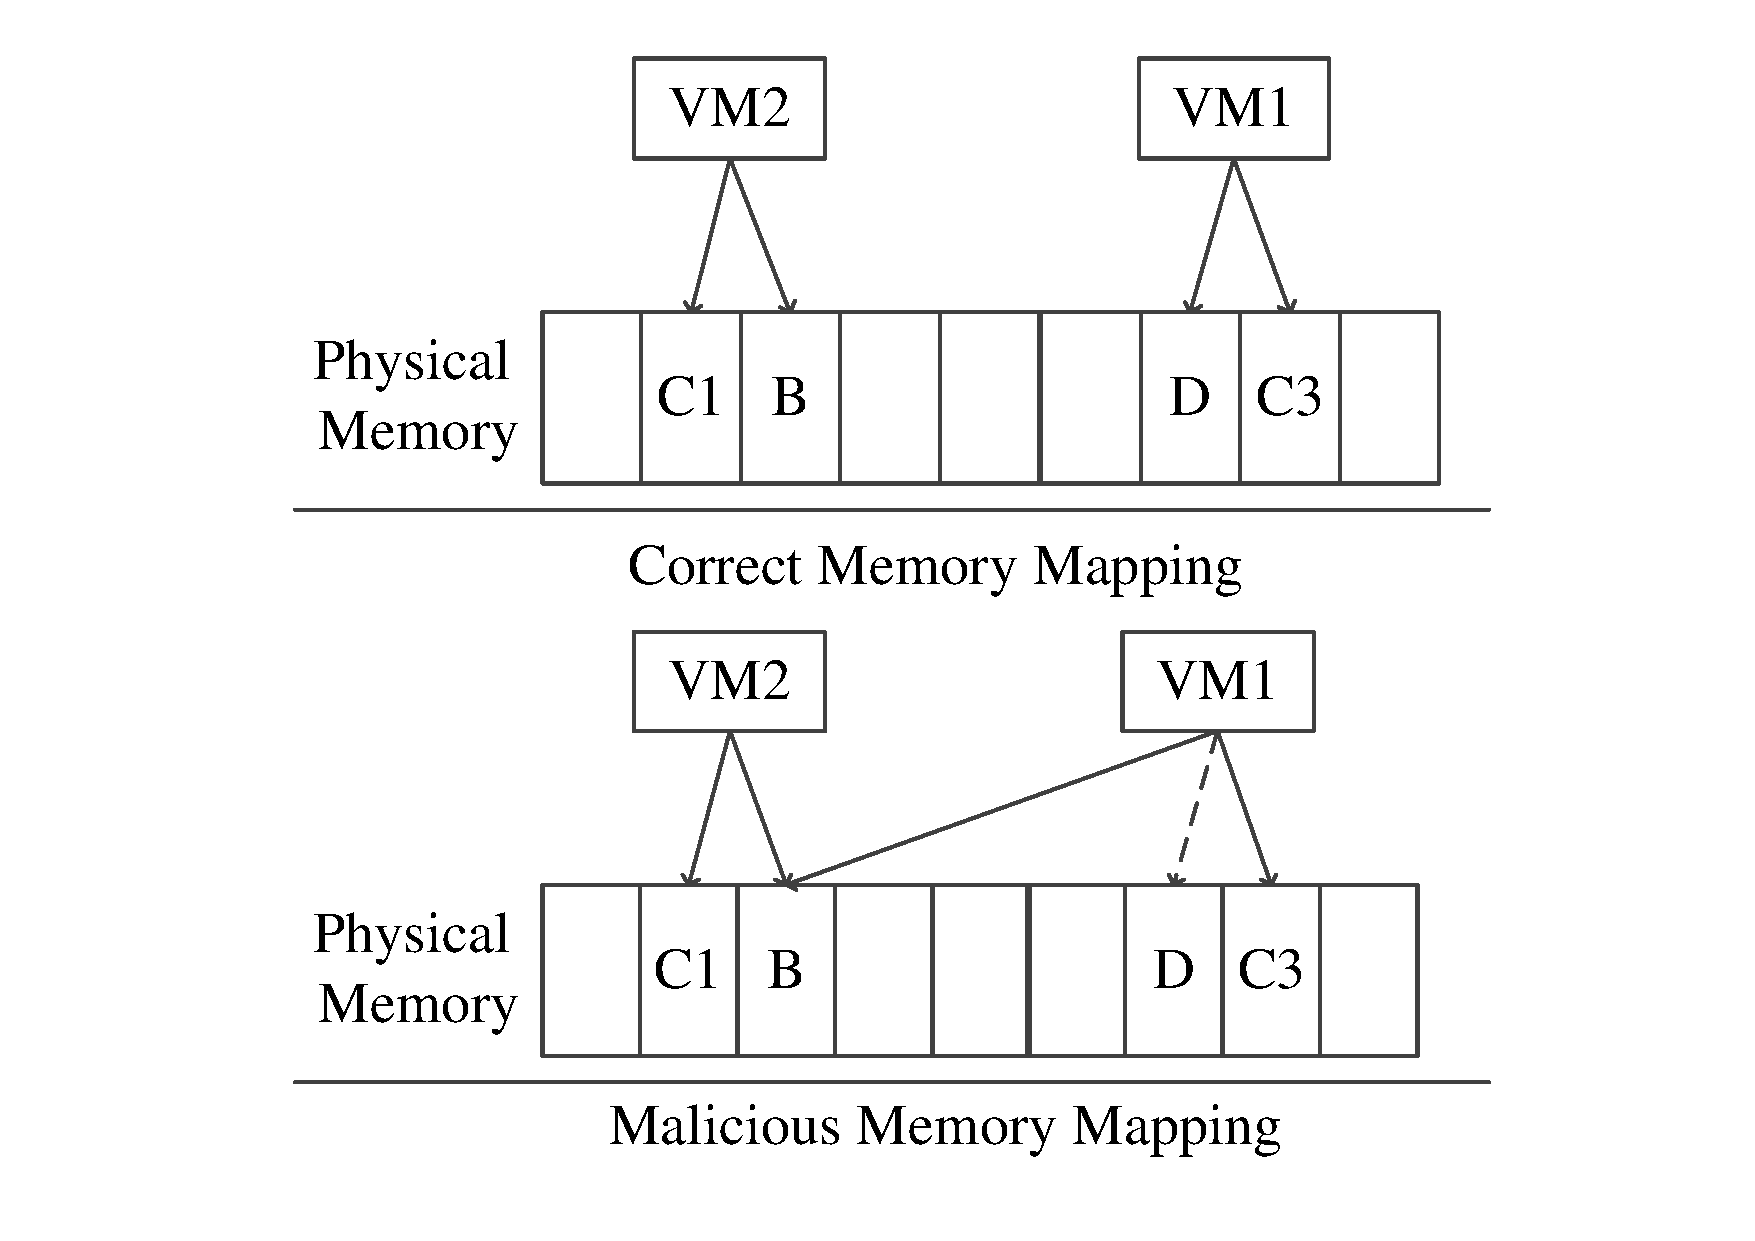
\includegraphics[width=10cm, height=6cm]{pdfvmcs.pdf}}%{pdfvmsm1.jpg}}
\caption{The execution process of double mapping. } \label{fig0}
\end{figure}

\textbf{Scene 2.}
    For the remapping attack, there are VM1 (attacker) and VM2 (victim). A physical page (named 'A') used by VM2 is released after it is used and it is released with VM2's content. After 'A' is released, VM1 remaps a GVA (named 'E') to 'A'. By this way, VM1 can access the content on 'A' used by VM2 through 'E', causing information leakage.
Through the analysis of these two kinds of attack models, it is necessary to achieve attack prevention.
\subsection{Assumption}

We propose some assumptions.
First, we assume hardware resources are trusted including processor, buses, BIOS, UEFI and so on, the trusted boot based on hardware can ensure the security and integrity of bootloaders. The TCB contains created HyperMI and hardware resources. Second, this paper does not consider denial of service attack (DOS), side channel attack and hardware-based attack, such as cold-boot attack and RowHammer. Third, we assume that there exists no software that runs at a higher privilege level than the hypervisor.


\section{Design and Implementation}\label{sec:design}



\begin{figure}
\centerline{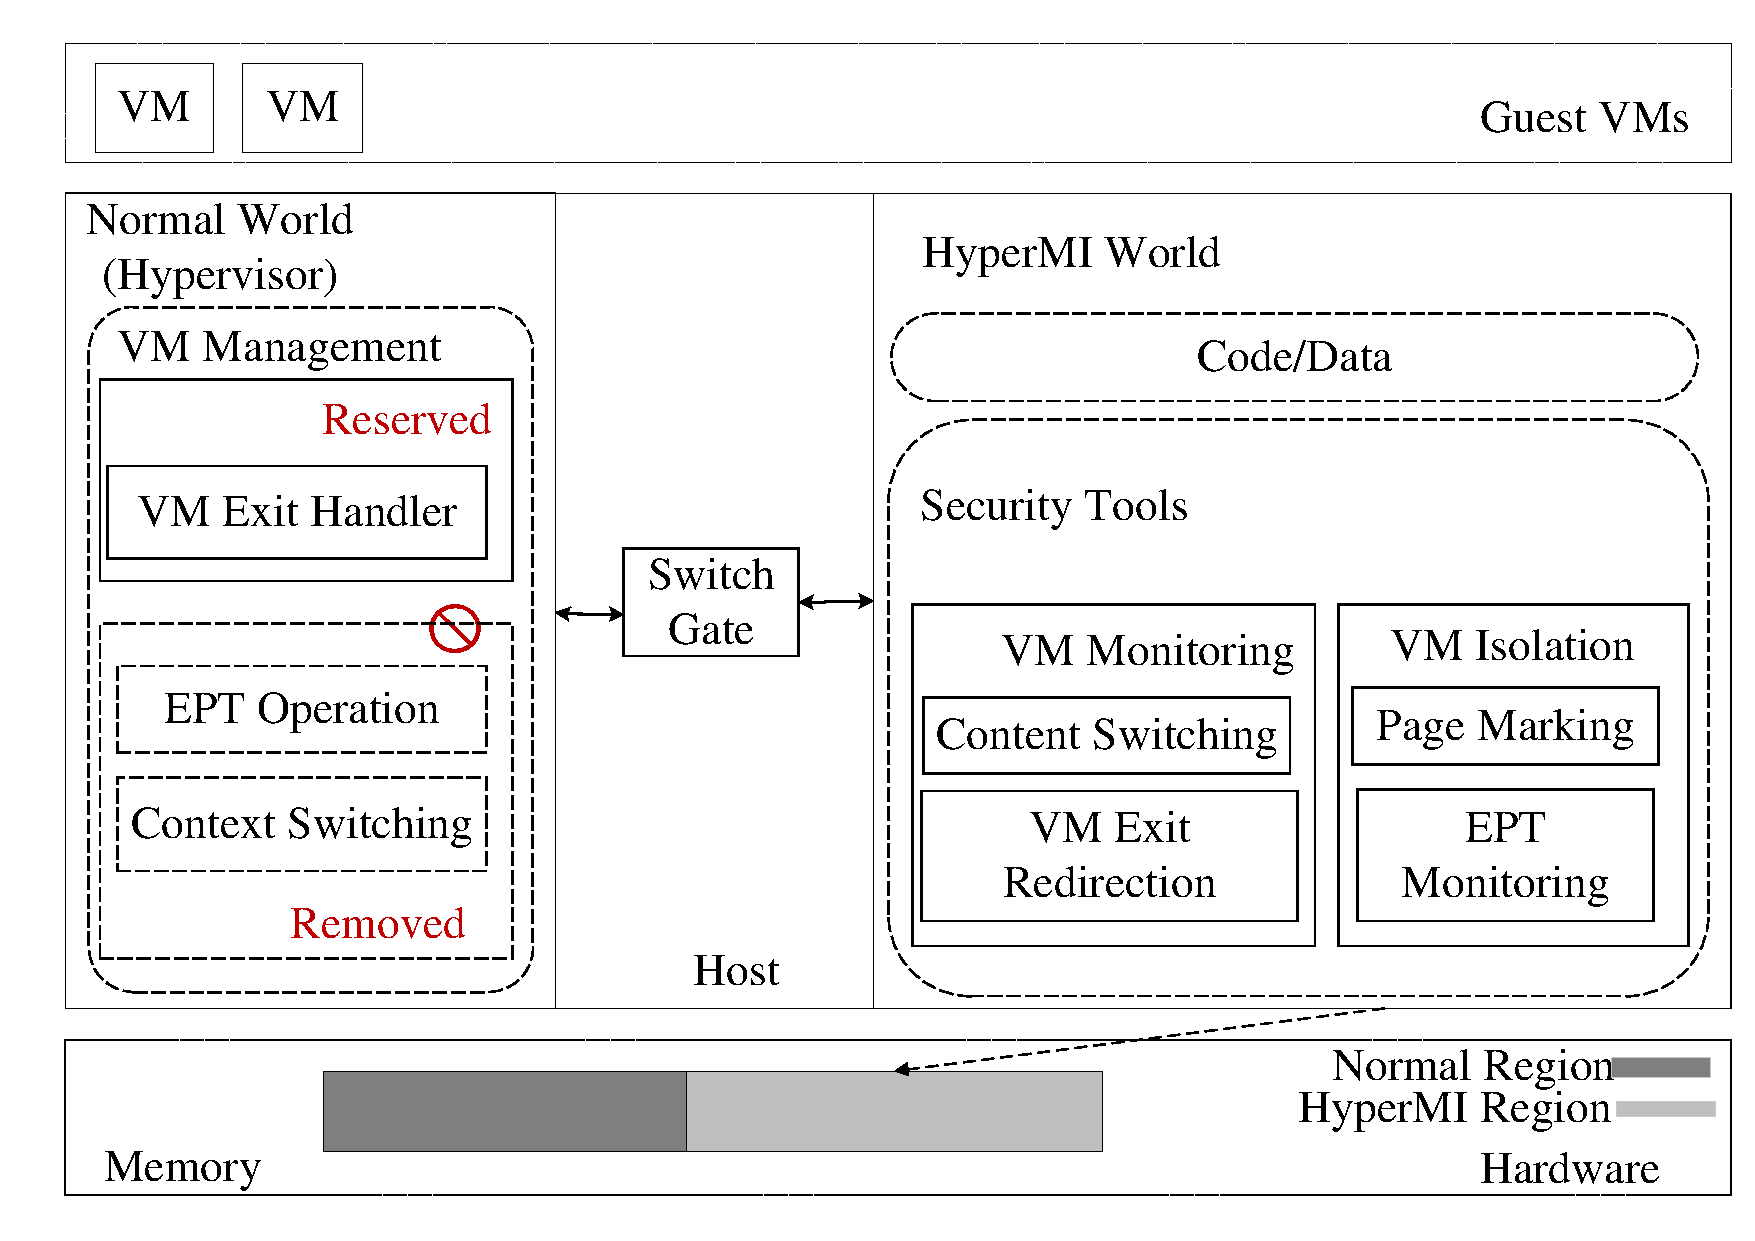
\includegraphics[width=9.5cm, height=7cm]{pdfvmcs1.pdf}}%{pdfvmsm1.jpg}}
\caption{The architecture of HyperMI. } \label{fig1}
\end{figure}

\subsection{Architecture} 
HyperMI is designed to provide a secure isolated execution environment to protect VMs against compromised hypervisor without depending on a higher privilege level software than the hypervisor or hardware.

Figure \ref{fig1} shows the architecture, the overall system contains three parts: several isolated VMs, hypervisor either in normal world or in HyperMI word, memory hardware including HyperMI region for HyperMI world and normal region for normal world.

The origin hypervisor is divided into two parts: HyperMI world which security tools can run in and normal world which hypervisor runs in. Firstly, HyperMI world is used to run security tools when hypervisor is compromised, so that these tools running in secure HyperMI world can resist attacks from compromised hypervisor. Secondly, operations for EPT and context switching module are deprived from normal world for security, then are put into HyperMI world, but VM exit handler module is reserved to handle VM exit in normal world. Thirdly, these two worlds can communicate with each other through the only secure channel, named Switch Gate. 


While the hypervisor together with guest VMs run in the normal world, the hypervisor is forced to request HyperMI to perform four operations on its behalf: 1) switching context between the hypervisor and VMs, 2) updating EPT of VMs, 3) verifying the pages when executing swapping operations to resist double mapping attack, 4) verifying the pages when executing releasing operations to resist remapping attack. After setting up the HyperMI, the whole system is ready to create isolated executing environment. With these designs, HyperMI enforces the isolation and protection of memory used by each VM. Furthermore, HyperMI guarantees security of interaction, memory isolation between the hypervisor and VMs.


\iffalse
\subsection{Interaction} \label{IN}


Figure \ref{fig+1} shows the interaction process of HyperMI. 
As described in the previous architecture, HyperMI is placed at the same privilege-level with the hypervisor, but in different address spaces. The two worlds interact through the channel, switch gate.


In the original system, only guest VMs and the hypervisor are involved during the execution. In details, 1) The guest VM would deliver a trap or receive an exception to interact with the hypervisor. 2) On receiving the VM exit signal, CPU would change to root privilege from the non-root privilege. During this process, hardware would save all guest context to VMCS data structure automatically. 3) The context of the hypervisor, that is saved in VMCS too, would be loaded into registers. Then exit handler in the hypervisor gets to run. 4) The hypervisor would call VMRESUME instruction to return 6the control flow to the halted VM when exit handler is finished. The context of the guest VM stored in VMCS (the context may be modified by the hypervisor during this process) would be loaded into register. 5) The guest VM resumes to run.

In HyperMI system, HyperMI hooks all functions which are involved in the interaction between the guest VM and the hypervisor. Besides, functions that are involved with EPT operation are also hooked to provide protection to EPTs. Therefore, the execution flow during VM exit has been changed on introducing HyperMI. The first two steps of VM exit are the same with that of the original system. For the third step, because the VMCS is protected by HyperMI, and the compromised hypervisor could not access this data structure. Thus, at the time, the functions used to read or write VMCS in the compromised hypervisor would be hooked and be redirected to HyperMI World, security checks would be performed to ensure the legal operation on them. It is the same with this process when functions that are involved with EPT are called. 
After the legal operations, HyperMI would transform control flow to the compromised hypervisor to perform VMRESUME. Because VMCS and EPT is perfectly isolated and secured from the compromised hypervisor, the compromised hypervisor cannot subvert guest VMs by modifying these two most crucial data structures.

\fi





\begin{figure}
\centerline{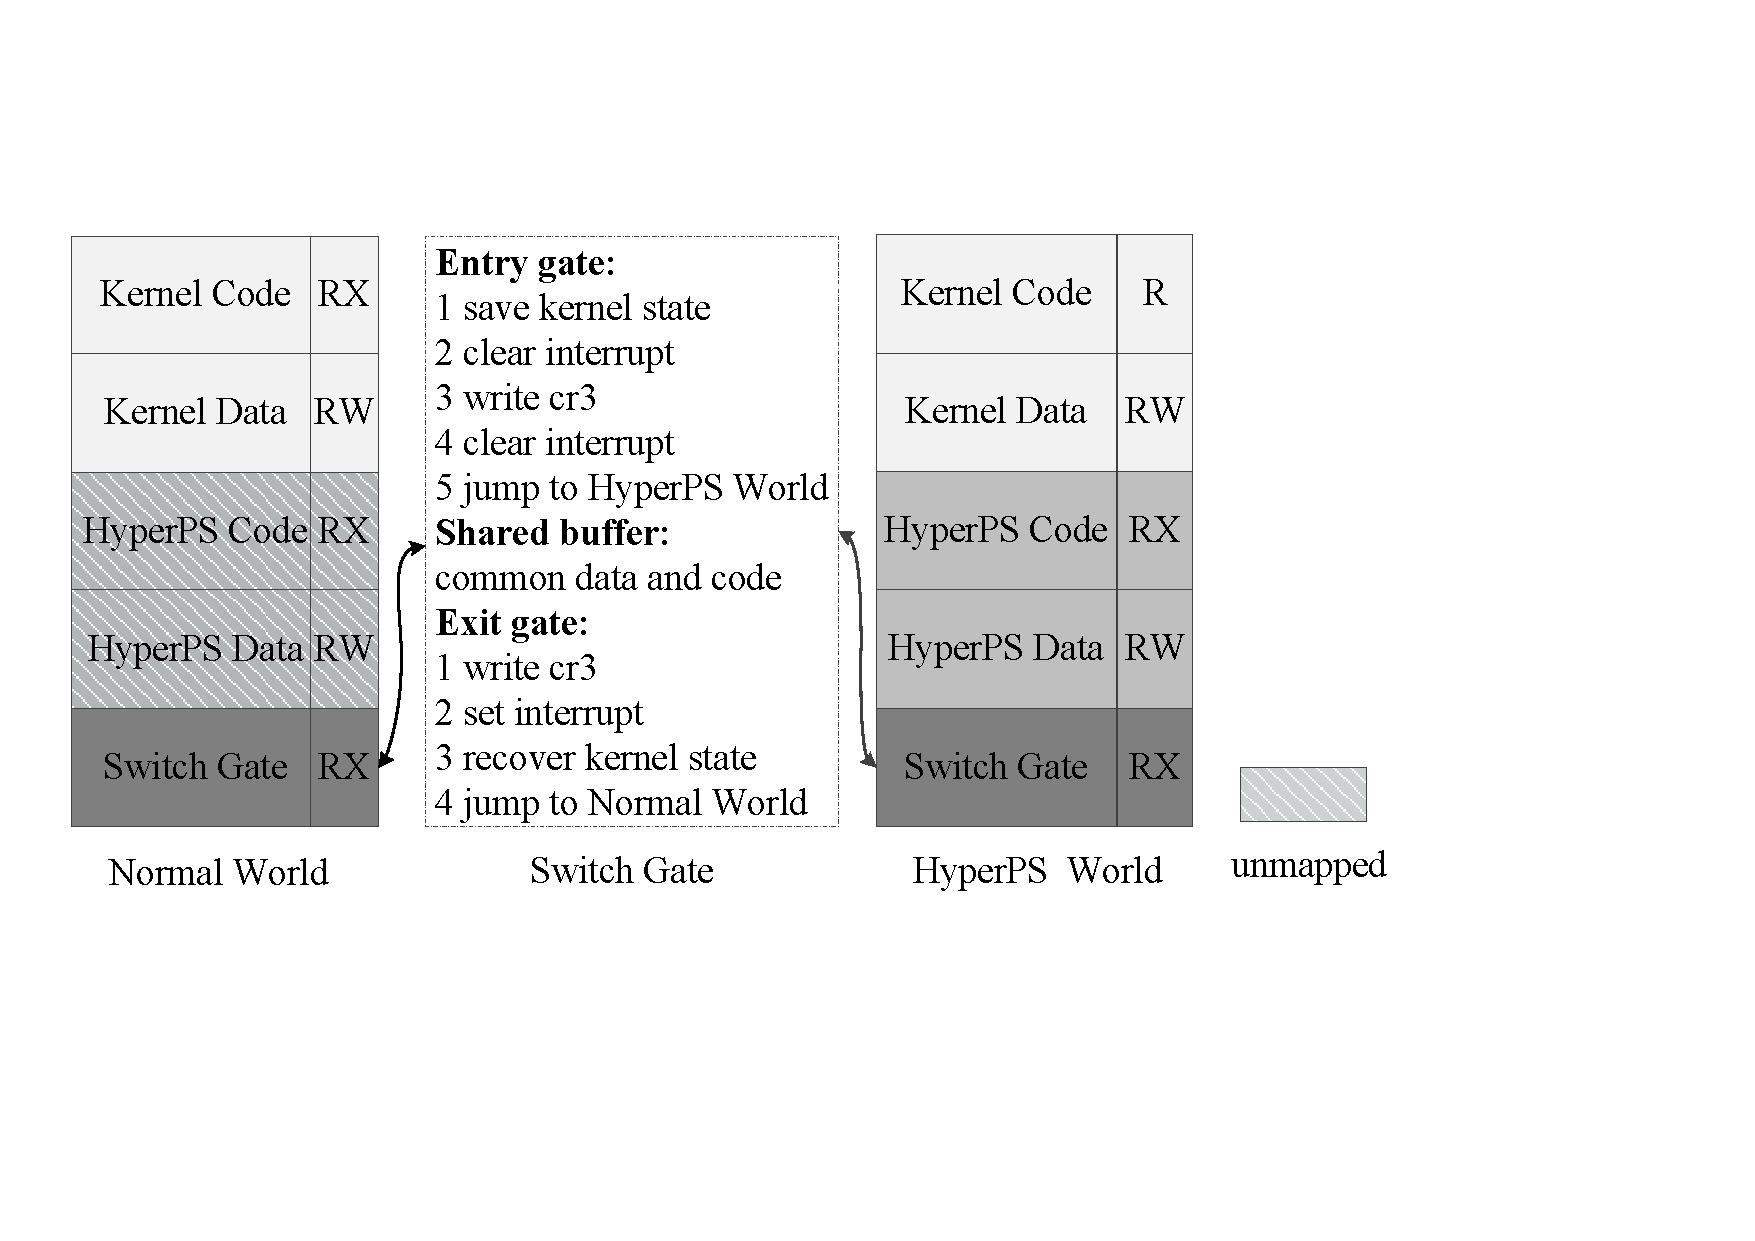
\includegraphics[width=11cm, height=7cm]{pdfvmcs2.pdf}}%{vmsm23.jpg}}
\caption{An overview of address space layout.} \label{fig2}
\end{figure}



\subsection{HyperMI World} \label {HWorld}

The creation of HyperMI World has two purposes: 1) creating an address space which can provide protection for key data and memory of VMs. 2) creating a software system that does not depend on hardware devices and adapts to multi-system platforms. The key point of its design is that it creates another address space at the same privilege-level with hypervisor. Unlike other same privilege-level software, HyperMI World depends on another new page table and two different address spaces.

\textbf{Creating HyperMI World}
 We use two isolated address spaces based on two sets of page tables to achieve isolation of HyperMI World.
Figure \ref{fig2} describes the address space layout of two worlds through two sets of page table, the normal page table and HyperMI page table. On the left of Figure \ref{fig2}, the normal page table contains code and data of the normal world except for that of HyperMI World. This can prevent compromised hypervisor from breaking the integrity of HyperMI World. Programs running in normal world can not access data in HyperMI World. On the right of Figure \ref{fig2}, all address is mapped in HyperMI page table.
HyperMI code remains executable and HyperMI data remains writable. What's the most important, kernel code is forbid to execute when HyperMI World is active, so that it can not attack HyperMI World.

\textbf{Creating Switch Gate}
In the middle of Figure \ref{fig2}, the switch gate includes entry/exit gate and shared buffer. Entry gate provides the only entrance to HyperMI World and the exit gate provides the address for returning to the normal world. The shared buffer contains common data and code in normal world and HyperMI World. Common code is switch code, common data is entrance address to HyperMI World and return address to the normal world. The switch gate is mapped at the same place in the normal world and HyperMI World because the switch gate code must be called by the two worlds before and after switching. Of course, the entrance address must be protected after switching to HyperMI World in case that a attacker accesses HyperMI World causally after trusted boot. This is introduced in section \ref{SG}.


\begin{figure}
\centerline{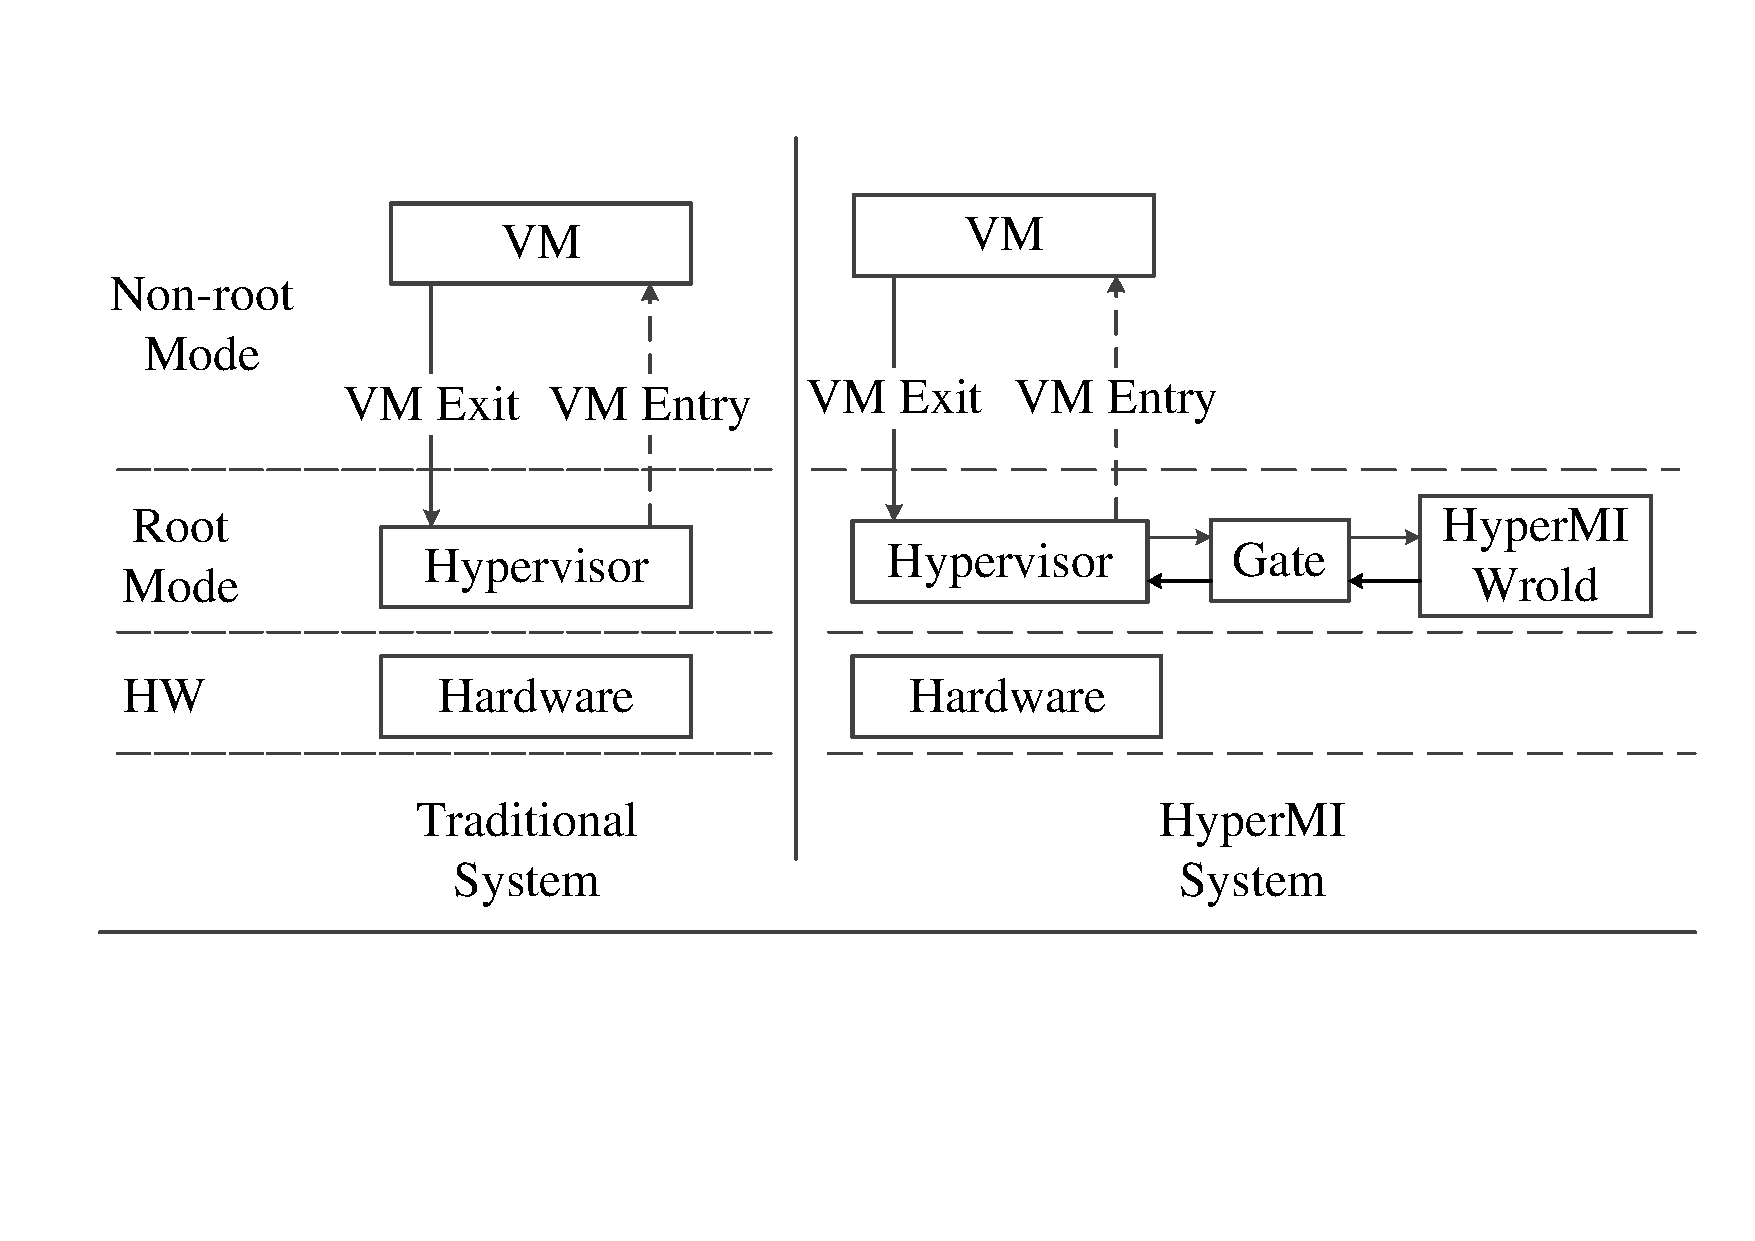
\includegraphics[width=9cm, height=7cm]{pdfvmcsProcess.pdf}}
\caption{Interaction comparison. } \label{fig+1}
\end{figure}


\subsection{VM Protection Approach}

\textbf{VM Monitoring}\label {interaction}
%Our approach takes advantage of the fact that, during the runtime of a VM,
 VMCS and EPT are the most two important data structures that the hypervisor can utilize to interact with the VM. And these two data structures can only be accessed by the hypervisor in traditional virtualization environment without HyperMI. If the hypervisor is compromised by an attacker, during the interval between VM Exit and VM Entry, some attacks can be conducted to subvert the VM. 

\textbf{VMCS Monitoring}
1) The compromised hypervisor can illegally get the address of VMCS and modify the content of VMCS directly. It can falsify the value of HOST\_RIP and execute control flow hijack attack.
2)It can also supply the VM with a dedicated illegal EPT by tampering the value of (EPTP) of VMCS. 
3) The compromised hypervisor can illegally modify the content of EPT entries. Because the EPT is responsible for managing all physical memory mapping of VM. The compromised hypervisor can easily conduct remapping or double mapping attack to the VM.
4) The attacker can load EPT of any VM and access the VM's normal memory illegally.

Hence, we straightforwardly provide the protection for these data structures by using HyperMI World. These two data are hidden in HyperMI World in case of malicious access from hypervisor. In specific, at each time when VM exits to compromised hypervisor, HyperMI catches these events and transfers VM Exit/Entry to HyperMI World. All functions that access VMCS and EPT entry are hooked and trapped into HyperMI World.
%, the modifying operations are conducted by precedures in HyperMI. 



%\textbf{Interaction Monitoring}
% \subsection{Interaction-data Monitoring}
%Given the importance of VMCS, HyperMI must isolate this data structure and achieve complte mediation to them. The compromised hypervisor should bot be able to bypass any HyperMI access control check. 
%First, Functions about creating and initing VMCS data structure are hooked into HyperMI. These functions are originally implemented by the hypervisor. HyperMI reconstructs these functionalities to ensure that the allocated VMCS is located in HyperMI World strictly. Operations that access to VMCS during the interval between VM Exit and VM Entry could not access the isolated VMCS data structure anymore, read and write operations are mediated and allowed only by legitimate HyperMI functionality.  
%Second, all functions, such as vmcs\_writel and vmcs\_readl, that would cause VM Exit to the hypervisor, are hooked into HyperMI World. Funtions about VM entry are hooked into HyperMI too. 
%Thus, HyperMI could not be bypassed in the process of contect switch between VM and the hypervisor. 
%The control flow of how HyperMI intermediate VM and the Hypervisor is depicted in Figure \ref{fig+1}.
%
%EPT is the other important data structure that should be protected by HyperMI. However, referring to the characteristics of EPT, only the write access functions to EPT should be hooked and intermediated by the HyperMI. 
%Given the importance of VMCS, HyperMI must isolate this data structure and achieve complte mediation to it.


%\textbf{VMCS Access Management}
%The protection for VMCS can not be ignored.
%% based on the fact that VMCS is structure recording all context information of the VM and it is managed by the compromised hypervisor. 
%%The VMCS structure always records the information of privileged registers, such as HOST\_CR3, EPT\_POINTER, HOST\_CR0, HOST\_CR4, VM\_EXIT\_MSR\_STORE\_ADDR, HOST\_RIP and so on. 
%During the VM entry or VM exit, the compromised hypervisor can tamper VMCS and execute following attacks: 1) Accessing memory region of VMCS directly. 2) Falsifying the value of HOST\_RIP, and the system will suffer control flow hijack. 3) Tampering the value of EPT\_POINTER(EPTP), and another malicious EPT is loaded. 4) Faking the value of HOST\_CR3, so the page table of host OS can be replaced.
We hide VMCS in HyperMI World to avoid access from hypervisor. 
In order to ensure that some functions (vmcs\_writel, vmcs\_readl et al.) can access VMCS properly, HyperMI hooks these functions into HyperMI World. So hypervisor requests HyperMI to handle operations about VMCS and return the corresponding result for the legal request. 

%In addition to hiding the address, HyperMI also intercepts and validates the execution of these instructions by placing hooks at these functions (vmcs\_writel, vmcs\_readl et al.). So hypervisor requests HyperMI World to handle operations about VMCS and return the corresponding result for the legal request.  
\iffalse
For the first kind of attack, to prevent compromised hypervisor accessing memory region of VMCS structure, HyperMI hides the base address of VMCS structure in HyperMI World. So, hypervisor loses the ability to access VMCS structure. In order to guarantee the normally running of original system, the hypervisor must require HyperMI to return the signal information rather than the real address on demand or trap the functions to HyperMI World, and avoid many functions about VMCS operations to access the address of VMCS structure directly. To avoid the last kind of attack, in addition to hiding the address, HyperMI also intercepts and validates the execution of these instructions by placing hooks at these functions (vmcs\_writel, vmcs\_readl et al.). So hypervisor requests HyperMI World to handle operations about VMCS and return the corresponding result for the legal request. 
\fi


%\textbf{VM Exit/Entry Management}
Since VMCS is hidden in HyperMI World, all context management (accessing VMCS operations) must be trapped to hypervisor. During VM Exit, hypervisor needs to access VM Exit reason data of VMCS, and then deal with the exit event.
%So in case of control flow makes mistakes
 Because hypervisor can not access VMCS, VM exit redirection is designed. The control flow jumps to HyperMI World to access VM exit reason data of VMCS structure, then switches to hypervisor and executes VM exit event handler function. VM Entry also accesses VMCS in HyperMI World. The control flow is shown as Figure \ref{fig+1}.


\begin{table}[htbp]
\centering
\caption{VM-Mark Table.}\label{tab1}
%\begin{tabular}{c|c|c|c}
\begin{tabular}{p{1.4cm}|p{1.2cm}|p{1.1cm}|p{1.7cm}}
\hline
\multicolumn{4}{c}{\bfseries\textbf\centering{VM-Mark Table}}\\
\hline
{\itshape\bfseries Label} & VMID & EPTID & EPT\_Address\\
\hline
{\itshape\bfseries Description} & { The VM Identifier} & The EPT Identifier & The Entry Address of EPT\\
\hline
\end{tabular}
\end{table}


\textbf{EPT Monitoring}
Some functions, EPT creating, loading, walking and destroying, need access address of EPT. It can cause system suspend if they can not access the address of EPT. In order to ensure these functions can execute normally, HyperMI places hooks on these functions, then dispatches them to HyperMI World and handles appropriately. In the meantime, HyperMI avoids double mapping attack to ensure that there is only one virtual address mapping to one physical memory page during EPT updating, and handles remapping problems to ensure the content of page cleaned after page is swapped out. This will be described in detail later.

If EPT isolation among VMs can not be guaranteed, a malicious VM can load other VM's EPT and access the memory data. It is important to ensure EPT isolation and one VM only access own corresponding EPT.
To ensure one EPT for one VM, HyperMI creates the VM-Mark structure stored in HyperMI World as Table 1 described. It records VMID, EPTID, EPT\_Address and binds them together. VMID is created when the VM is created. 
%and destroyed based on hash value of the image of VM.
 EPTID and EPT\_Address is recorded as long as the EPT of current VM is created.


%EPT is the other important data structure that should be protected by HyperMI. However, referring to the characteristics of EPT, only the write access functions to EPT should be hooked and intermediated by the HyperMI. 
%With Intel VT-x technology, operations about address translation, such as loading the ept address and walking the requested address, are completed by the hardware automatically. The hypervisor would not alter any EPT entry in this process. However, all functions such as EPT creation, destroyment, modification that associated with write operation to EPT entry, are hooked into HyperMI. HyperMI reconstructs all these functions and integrity protection approaches with them. For a instance, HyperMI enhance the security policy that the virtual address can only be mapped to one physical address. This security policy, as a result, could prevent \textbf{Double Mapping} attack at the isocated execution environment. \textbf{Remapping} attack is also be countered by the reconstructed EPT management functions in HyperMI. 
%
%In commercial cloud environment, On the one hand, there would more than one VM are managed by one same hypervisor. Hence, It is also much important to guarantee the associated relationship between EPT and their VM. On the other hand, Because all VMs share the same physical memory, a malicious VM can load other VM's EPT and access the memory data. It is important to ensure EPT isolation and one VM only access own corresponding EPT.
%%Intercepting the loading EPT operation and verifying the correctness of EPT can avoid loading a wrong EPT and leaking the content of physical memory page. 
%To ensure one EPT for one VM, HyperMI creates the VM-Mark structure stored in HyperMI World as Table 1 described, and record VMID, EPTID, EPT\_Address and binds them together. VMID is created and destroyed based on hash value of the image of VM. EPTID and EPT\_Address is recorded as long as the EPT of current VM is created.

\begin{figure}
\centerline{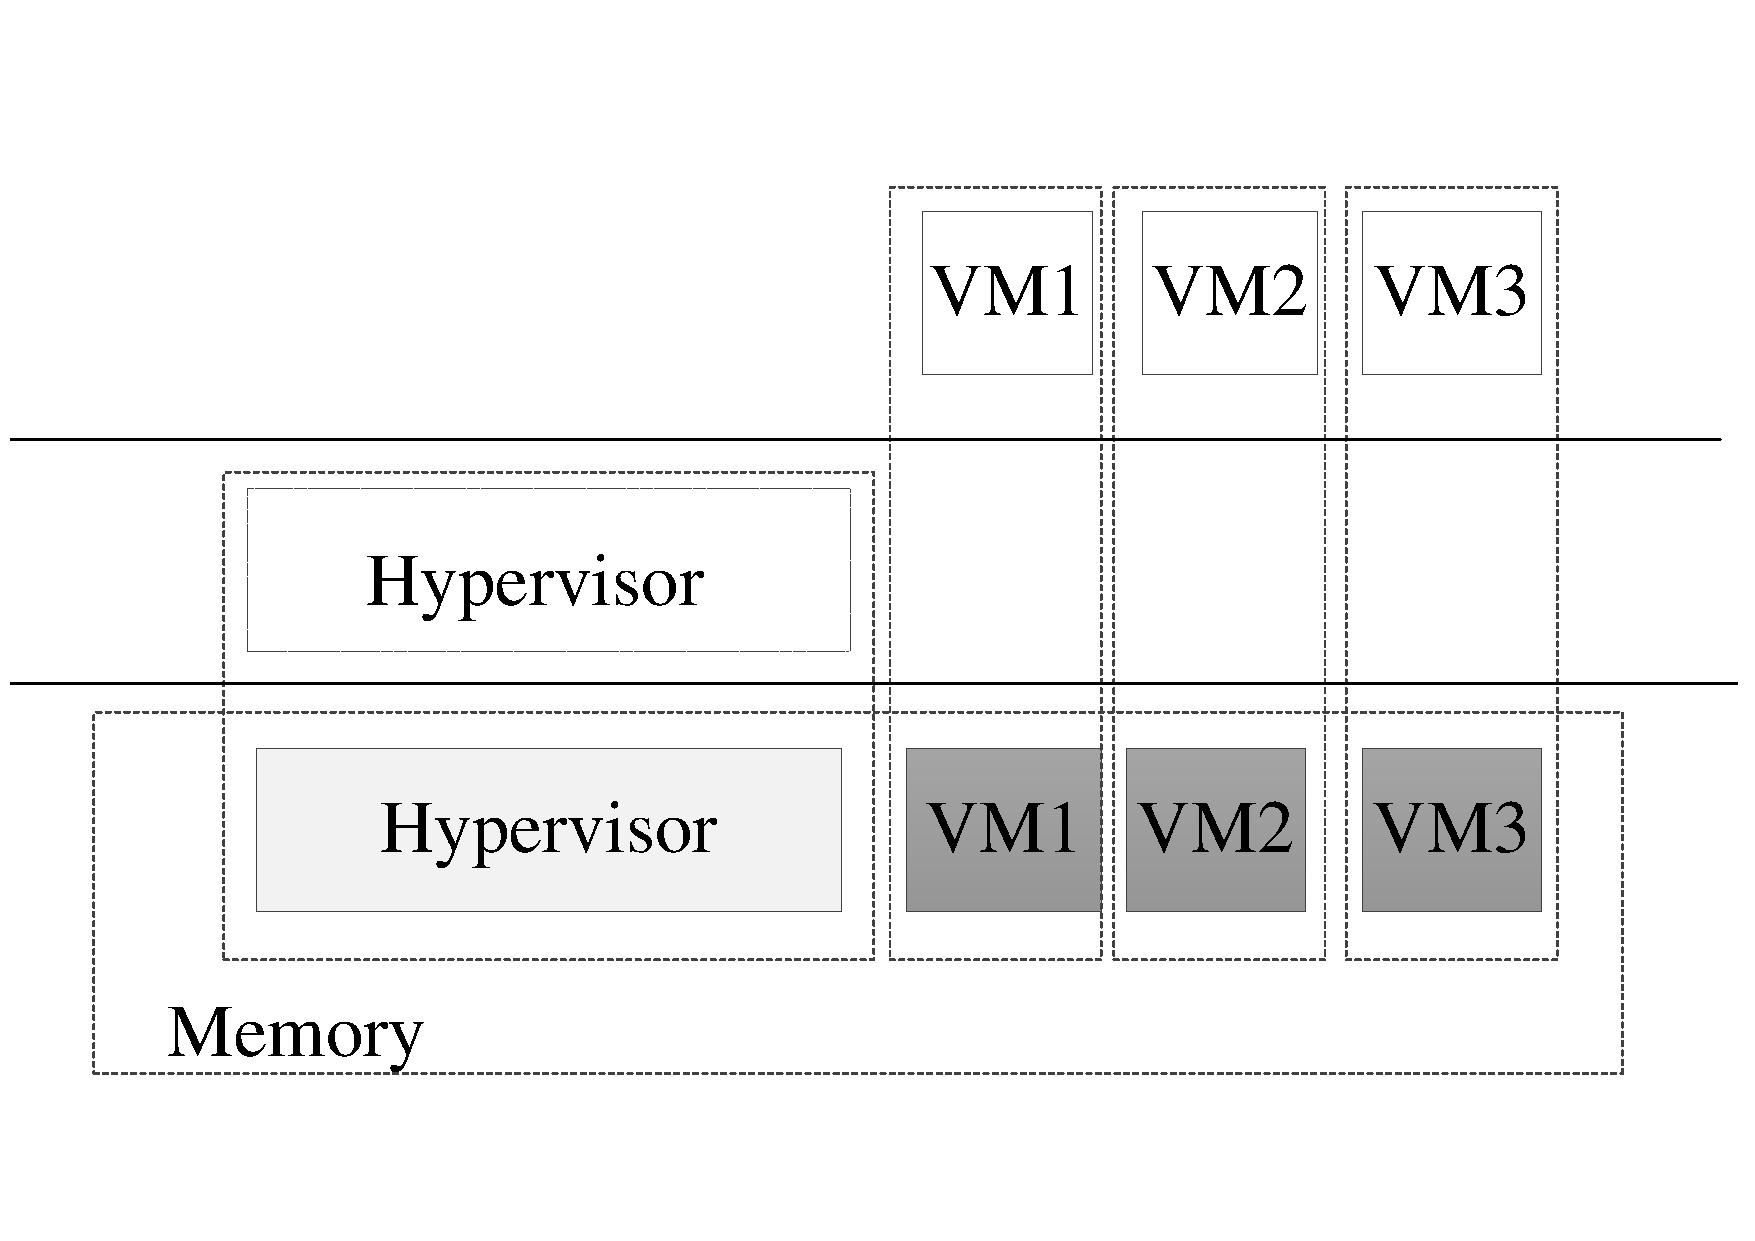
\includegraphics[width=7cm, height=4cm]{pdfvmcs3.pdf}}%{vmsm32.jpg}}
\caption{Memory isolation for VMs.} \label{fig3}
\end{figure}


\textbf{VM Isolation}
Isolating memory is another aspect that should be considered. We need to ensure that the VM and the hypervisor can only access their own corresponding memory, as shown in Figure \ref{fig3}.
Without memory isolation, a VM may suffer double mapping attack and remapping attack described in section \ref{threat}. We use Page-Mark structure described in Table \ref{tab2} to record the owner and status of every page. 

\begin{table}
\centering
\caption{Page-Mark Table.}\label{tab2}
%\begin{tabular}{|c{1cm}|c|c|}
\begin{tabular}{p{1.2cm}|p{1.4cm}|p{1.5cm}}
\hline
\multicolumn{3}{c}{\bfseries\textbf\centering{Page-Mark Table}}\\
\hline
{\itshape\bfseries Label} & OwnerID & Used \\
\hline
{\itshape\bfseries Description} & The Owner Identifier & Free or Used \\
\hline
\end{tabular}
\end{table}

In order to go against the double mapping attack in the process of EPT updating, HyperMI should finish these two tasks: 1) It should verify the owner of pages when EPT updates. 2) It should mark the OwnerID field of Page-Mark structure for unused pages or thwart the mapping operation for used pages in case of malicious double mapping behavior. So page marking technique can divide all the pages into different catalogs: the pages of hypervisor or the pages of every VM.

To go against the remapping attack, HyperMI cleans the content of the page when the page is swapped out, so attackers can't get the content of the page by the way of remapping. HyperMI clears the Page-Mark structure of the corresponding page. 





\subsection{Security Guarantee for HyperMI World}\label {SG}
The security of HyperMI World guarantees the security of HyperMI, because HyperMI relies on HyperMI World to provide a secure execution environment.
Nevertheless, without any protection measures, the normal world kernel page table is not secure for four reasons: 1)Attackers can control page table with the highest privilege after hypervisor is compromised. 2) Attackers can bypass the switch gate to break the security of HyperMI World. 3) Attackers with the highest privilege can free to execute privileged instructions to access the value of privilege registers, such as CR0, CR3 and so on. 4) Attackers can carry out DMA attack to access HyperMI World casually.
We detail the protection measures for these four types of attacks below.
%\paragraph



\textbf{Protecting Page Table}
There are three reasons for controlling the two sets of kernel page tables: 1) To access casually or bypass HyperMI World, the attacker can tamper normal page table to map address of HyperMI World or load malicious page table to CR3.
%2) To execute code injection attack, the attacker can close the write protection mechanism by modifying the value of CR0 register, changing the access permission bits of the memory page. 
2) The attacker can cover the hooked functions, redirect the functions to malicious code and bypass interaction monitoring of HyperMI. 3) To break HyperMI World, malicious kernel code with execution permission can be executed to subvert HyperMI.
% by means of the vulnerabilities of the original kernel code. 
%access HyperMI World causally when HyperMI World is running if kernel code has the execution permission. 
%Therefore, three secure approaches against these attacks are as follow.

For the first attack, %HyperMI code and data is unmapped in page table of normal world.
% And to protect the entrance address to HyperMI World from being leaked,
%pre-allocate some space during trusted boot which kernel can't access directly through MMU, critical data in
we remove all entries that map to HyperMI World from the page table in normal world. Deprive the ability to access CR3 of the kernel. % in order to avoid loading illegal page table, and resist bypassing HyperMI World.
For the second attack, we intercept the accessing operation to CR0 and maintain the WP bit as 1. We stick to W$\oplus${X} and maintain the code segment of hooked functions unwritable.
For the third attack, we set the kernel code segment as NX (non-executable) when HyperMI World is running. For more security, we modify the kernel to configure these two sets of page table as read-only by setting the memory regions of the page tables unwritable. This is necessary to prevent the page tables from being modified by attackers. Any write permission modification of two sets of page table must cause the kernel to page fault, then we dispatch page fault to HyperMI World to verify the correctness of address mapping. 
%This idea is adopted in SKEE\cite{Azab2016SKEE}.


\textbf{Worlds Switching Securely}
HyperMI creates a switch gate between the normal world and HyperMI World by loading entry address of page table into CR3.
In order to ensure switch security, we design the switch process as follows.
% And we must ensure atomicity and security during the switching process.

The switching process described in Figure \ref{fig2} is as follows: 1) Save the kernel state to the stack including general registers and interrupt enable/disable status. 2) Clear the interrupt with the CLI instruction. 3) Load the page table to the register CR3. 4) Interrupt again. 5) Jump to the HyperMI World. For the exit process, the control flow returns to the normal world by performing the operations in the reverse order.

\iffalse
If we don't use the switch process above, just write the address of different page tables to CR3. Switch to HyperMI World and return to normal world directly. Attackers can attack the system by violating security. Attackers can get the address of HyperMI World by accessing the register CR3. We use interruption policy (the first step) in our switching process to prevent this attack. 
If there is not the second interruption (the fourth step), attackers can implement another attack. They can jump the first interruption.
%and get the base address of page table of HyperMI World from CR3. 
Then they can access HyperMI World successfully. 
%This attack can go against security and atomicity.
However, we adopt twice interruption policy (the fourth step) in our switching process to prevent this. 
%Twice interruption is used to ensure security in case of attackers carrying out attack after the third step in our switch process. 
%After attackers jump the first interrupt and get the address from CR3, the second interruption can prevent attackers going to HyperMI World directly. 
This idea is inspired from the design of gate in SecPod\cite{Wang2015SecPod}.

\fi

\textbf{Accessing Privilege Registers Securely}
The hypervisor without HyperMI is privileged and it can free to execute privileged instructions, so that it can write any value to the related privileged registers. 1) Malicious attackers can close DEP mechanism by writing CR0, close SMEP mechanism by writing CR4. 2) Kernel code can load a crafted page table to bypass HyperMI World by converting a meticulously constructed address of one page table to CR3.
To prevent the attack, HyperMI deprives sensitive privilege instructions executed by the hypervisor, and dispatches captured events to HyperMI World. HyperMI World can choose how to handle this event, such as executing, issuing alerts or terminating the process. 

\textbf{Resisting DMA Attack}
%Thirdly, it is important to focus on DMA attack. 
DMA operation is used by hardware devices to access physical address directly. Malicious attackers can read or write arbitrary memory regions including HyperMI World by DMA. Therefore, it is a crucial focus of intercepting direct access to physical pages belonging to HyperMI World by DMA operation. 
Fortunately, HyperMI employs IOMMU mechanism to avoid DMA attack, which can carry out access control for DMA access. Our approach adopts two policies: 1) We remove the corresponding mapping of the critical data from the page table which IOMMU uses. These critical unmapped data includes the entrance address of HyperMI, data recording Page-Mark structure used in VM memory isolation, VM-Mark structure used in EPT management and so on. 2) HyperMI intercepts the address mapping functions about I/O, verifies whether the address belongs to an address space of HyperMI World, then chooses to map or unmap.


Through the above security measures, HyperMI can be protected from being bypassed and being breaking, thus providing a secure execution environment for VM protection.




















\iffalse
\section{Implementation}\label{sec:imp}

HyperMI is implemented on x86 platform based on KVM hyervisor (version 3.10), both the host and guest run Linux. In the following, we present details of the prototype. 

\subsection {HyperMI Initialization}
An essential requirement during system initialization is only allowing to load the hypervisor and HyperMI into the platforms.
The initialization of HyperMI includes the creation of HyperMI World, the hooks of key functions used to monitor as well as the creation of Page-Mark table and VM-Mark table. 

First, as required by HyperMI, HyperMI World is created to provide a trust execution environment. The permission for the kernel code is non-execution when HyperMI World is active. 
Second, when the hypervisor boots up, the hypervisor has to trap to HyperMI to initialize its critical data including MMU, system control registers, VMCS and EPT. These data access functions are described in table \ref{tabhook}.
Third, these functions are like triggers, and once the relevant critical data is accessed, these operations are hooked to HyperMI World to execute. 
Finally,HyperMI also examines every page table of hypervisor to confirm that the entry address of HyperMI World are not existed in the hypervisor's address space. 
Finally, HyperMI updates Page-Mark table to reflect the current memory status and owner. It creates VM-Mark table to blind VM and EPT.


\subsection {Interaction}

A VM can not handle the operation of privileged instructions and need the assistance of hypervisor, so they interact through the VM Exit/Entry. Because interaction data, VMCS structure, is stored in HyperMI World, the operation of accessing VMCS structure is trapped in HyperMI World, so VM Exit/Entry control flow is changed. The control flow as follows. 1) VM sends out exit signal to hypervisor. 2) After receiving signal, hypervisor notifies CPU to write the value of system registers to VM status data of VMCS structure, and to write host status data of VMCS structure to system registers. 3) Control flow jumps to HyperMI World to access VM exit reason data of VMCS structure, switches to hypervisor and execute VM exit event handler function. 4) VM Exit finishes.
VM Entry also requires access to VMCS in HyperMI World rather than in normal world. The control flow is opposite to that of VM Exit.

\subsection {Page Mapping}

To allocate a physical page to a VM, HyperMI must update the relevant address translation of the EPT.
Before executing EPT update, the key step for memory isolation is to check the usage state of the mapping page. 
By checking the Page-Mark table, HyperMI can keep the page away from being owned by multiple owners. If the page is allocated for the first time, HyperMI sets the OwnerID and Used flag of Page-Mark table and updates the corresponding EPT entry. Meanwhile, release this page from the address space of hypervisor. Otherwise, this request fails and page can not be allocated successfully. In this way, HyperMI prevents a compromised hypervisor from executing any double mapping attack to the page already allocated to other owners.


\begin{table}
\centering
\caption{Hooked Functions.}\label{tabhook}
%\begin{tabular}{|c{1cm}|c|c|}
\begin{tabular}{p{1cm}|p{1.2cm}|p{1.1cm}|p{1.4cm}|p{1.6cm}}
\hline
\multicolumn{5}{c}{\bfseries\textbf\centering{Hooked Functions}}\\
\hline
{\itshape\bfseries Structure} & Page & Regs & VMCS & EPT \\
\hline
{\itshape\bfseries Functions} &page fault & cr0\_write cr3\_read cr3\_write cr4\_write & vmcs\_readl vmcs\_writel & ept creation ept loading ept walking ept destroying \\
\hline
\end{tabular}
\end{table}

\subsection {Page Unmapping}

To deallocate a physical page from a VM, HyperMI clears the appropriate EPT to invalidate this mapping. In addition, HyperMI clears the content of this page before resetting the Used flag of Page-Mark table. Clear the OwnerID field and set Used flag to be free. With this approach, page reuse attacks and remapping attacks are prevented.
\fi


\section{Evaluation}\label{sec:evaluation}
%We describe the design and implementation of HyperMI. 
%In this section, we evaluate the protection effectiveness and performance of HyperMI by exploiting vulnerabilities and comparing it with traditional KVM through a set of benchmarks.
In this section, we first analyze the security guarantees provided by HyperMI. Then, we evaluate the performance overhead by running a set of benchmarks on both standard KVM and HyperMI.



\subsection{Security Analysis}
 
%In section \ref{sec:design}, we discuss in detail how HyperMI achieves memory isolation, and secure interactions between VM and the hypervisor. Just as the threat model described in the section \ref{threat}, an attacker could subvert the upper VMs by conducting attacks such as cross-domain attack with a malicious virtual machine.
In this section, we elaborate the security evaluation on how HyperMI achieves memory isolation among VMs through the monitoring interaction data. 
In addition, we analyze the security of HyperMI itself. Table \ref{tab3} shows the real attack instances in line with the above attack model. 

%However, these two attack vectors, regardless of their attack path, both focus on critical interaction data and data on memory, afterwards, modifying more detailed data, such as the VMCS data structure, EPT and EPT Pointer. Thus, we will elaborate on how HyperMI fends of these attack, and Table \ref{tab3} shows the two real attack instances in line with the above attack model. 
% the attack instances listed in Table \ref{tab3} perfectly match the description of attacker, so we will use these two instances to specifically analyze security performance. 


\textbf{Modifying Interaction-Data Attack}
We clarify interaction data including VMCS in Section \ref{interaction}.
 To prevent interaction-data leakage, we protect VMCS from the attacker. Firstly, VMCS is hidden in HyperMI World and can not be accessed by hypervisor. Secondly, functions that can access VMCS are hooked into HyperMI World, therefore, no functions outside HyperMI World can access VMCS. The attacker can not get location of VMCS and access it. This prevents attackers from tampering interaction data attacks. We examine protection for VMCS by conducting several attack cases which are widely adopted in real world. Table \ref{tab3} lists all attack cases we used. The attack, named Interaction-data attack, tries to tamper the Guest\_CR3 field in VMCS. This attack fails because it can not access VMCS. 
% The experimental results show that the access failed, malicious interaction-data accessing is prevented successfully.
  According to the above analysis, the attacker can not access VMCS, and can not conduct further attacks. Therefore, the VM interaction data can be protected by HyperMI.
  %cannot be modified. 


%CVE-2009-2287 allows attacker to provide invalid value of CR3, which is an important data value in VMCS data structure. Because HyperMI would check the value of CR3 before VM entry instruction is conducted, an attacker has no chance to load the value to physical CR3 register successfully. HyperMI protects all important data values in VMCS data structure. In details, interaction between hypervisor and VMs runs in HyperMI World, VMCS structure used to record context switching data is hidden in HyperMI World, so an attacker cannot modify VM states during context switching. HyperMI adopts VM-Mark table to ensure that load consistent EPT for every VM, so attacker cannot modify EPTP. Therefore, the VM states cannot be modified. 




\textbf{Subverting Memory Across VMs Attack}
%A kind of attack is subverting memory protection across VMs. 
%Original hypervisor manages the memory of VM through EPT which controls the address translation of VM, so compromised hypervisor can incur malicious memory access attack, such as double mapping attack and remapping attack. However, HyperMI hides the address of EPT in HyperMI World and hooks all operations about EPT into HyperMI World. Page tracking technology can make and prevents double mapping and remapping attack. Page tracking technology can ensure that each physical page has only one owner, verify the ownership of each physical page when EPT updates the mapping, and ensure the safe mapping of physical memory. Page tracking  technology can clear the contents of pages when they are completely released, ensuring information security.
%
The main attacks that attackers can execute on subverting memory are double mapping attack and remapping attack.
Firstly, double mapping attack succeeds by allocating memory pages that have already been owned by a hostile VM to a victim VM. Page marking and write-protection of EPT prevent this kind of attack. For each new mapping to a VM, HyperMI validates whether the page is already in use according to Used field of Page-Mark structure. Meanwhile, the allocated pages must be marked in the Page-Mark table for tracking. Secondly, another challenge is page remapping attack by a compromised hypervisor from a victim VM to a conspiratorial VM. This attack involves remapping a private page to another address space. To defeat this type of attack, HyperMI ensures that whenever a page is released, its content must be zeroed out before creating a new mapping.


We implement a real attack, CVE-2017-8106 in kernel version 3.12. A privileged KVM guest OS user accesses EPT, conducts attacks via a single-context INVEPT instruction with a NULL EPT Pointer. Attackers can not implement successfully and incur EPT access fault because HyperMI hides the address of EPT in HyperMI World and hijacks the loading of EPT. HyperMI verifies the value of EPT to avoid load NULL value. Therefore, HyperMI can avoid subverting memory across VMs including double mapping attack, remapping attack as well as malicious EPT access.
% attacker is unable to subvert the upper VMs by exploiting the hypervisor vulnerability. 
%But an attack on memory is not limited to loading malicious EPT Pointer.


\begin{table}
\centering
\caption{Hypervisor Attacks Against HyperMI.}\label{tab3}
\begin{tabular}{p{2.8cm}|p{5.5cm}}
\hline
{\itshape\bfseries Attack} & {\itshape\bfseries Description} \\
\hline
Interaction-data Attack & Load a crafted GUEST\_CR3 value\\
\hline
CVE-2017-8106 & Load a crafted EPT value \\
\hline
DMA Attack & Access HyperMI World by DMA \\
\hline
Code Injection Attack & Inject code and cover hooked functions to bypass HyperMI World \\
\hline
\end{tabular}
\end{table}

\textbf{Destroying HyperMI World}
HyperMI is created by relying on page tables.
% When HyperMI does not work, the original kernel with high privileges can access any page tables and modify them. It can also access control registers casually, redirect hooked functions used to monitor previously, and even maliciously destroy HyperMI World through DMA. 
We analyze the protection of HyperMI World from four aspects, page table modification attack, hooks redirection attack, reg modification attack and DMA attack.


\subsubsection{Page Table Modification Attack}

Page table protection has been introduced in section \ref{SG}. The entry address mapping of the HyperMI World page table is deleted from the old page table to prevent the kernel from accessing HyperMI World directly through the page table mapping. When HyperMI World is active, the kernel code does not have any executable permissions in case of attacking running processes in HyperMI World. An attacker may attack in two ways.
First, the attacker may try to directly access the new page table address on the kernel page table by virtual address mapping. When he accesses it, there is page fault due to the absence of address mapping.
Second, the attacker may run kernel code while HyperMI World is active to attack programs running in HyperMI World. This can be prevented because of the absence of executable privilege of kernel code.



\subsubsection{Hooks Redirection Attack}

Due to the code of hooked functions including VMCS operations, EPT operations and control register access operations is writable-protection. Accessing CR0 register operation used to set W$\oplus${X} is controlled and page table updating used to change code execution privilege is limited, the attacker can not redirect hooked functions and bypass monitoring.

\subsubsection{Reg Modification Attack}

Some registers access operations including CR0, CR3, CR4, are controlled and hooked to HyperMI World. CR0 register can control the W$\oplus${X} privilege of code, CR3 can control the loading of the page table and CR4 can decide SMEP mechanism. Protection for page table, hooked functions and regs, plays a role mutually in protection for HyperMI. 

\subsubsection{DMA Attack}

%In addition, the memory can be accessed through DMA operations bypassing the MMU, except for accesses by executing memory accessing instructions.
 DMA attack is described in detail in section \ref{SG}. Attackers can use this feature to read or corrupt arbitrary memory regions. DMA attack is not a threat to HyperMI, because HyperMI is inherently secure against DMA using IOMMU. Remove the corresponding mapping of the critical data from the page table which IOMMU uses. These critical unmapped data includes the entrance address of HyperMI, data recording Page-Mark structure used in VM isolation, VM-Mark structure and so on. DMA attack that aims at modifying the VM memory or the page tables can also be defeated.

\begin{figure}
\centerline{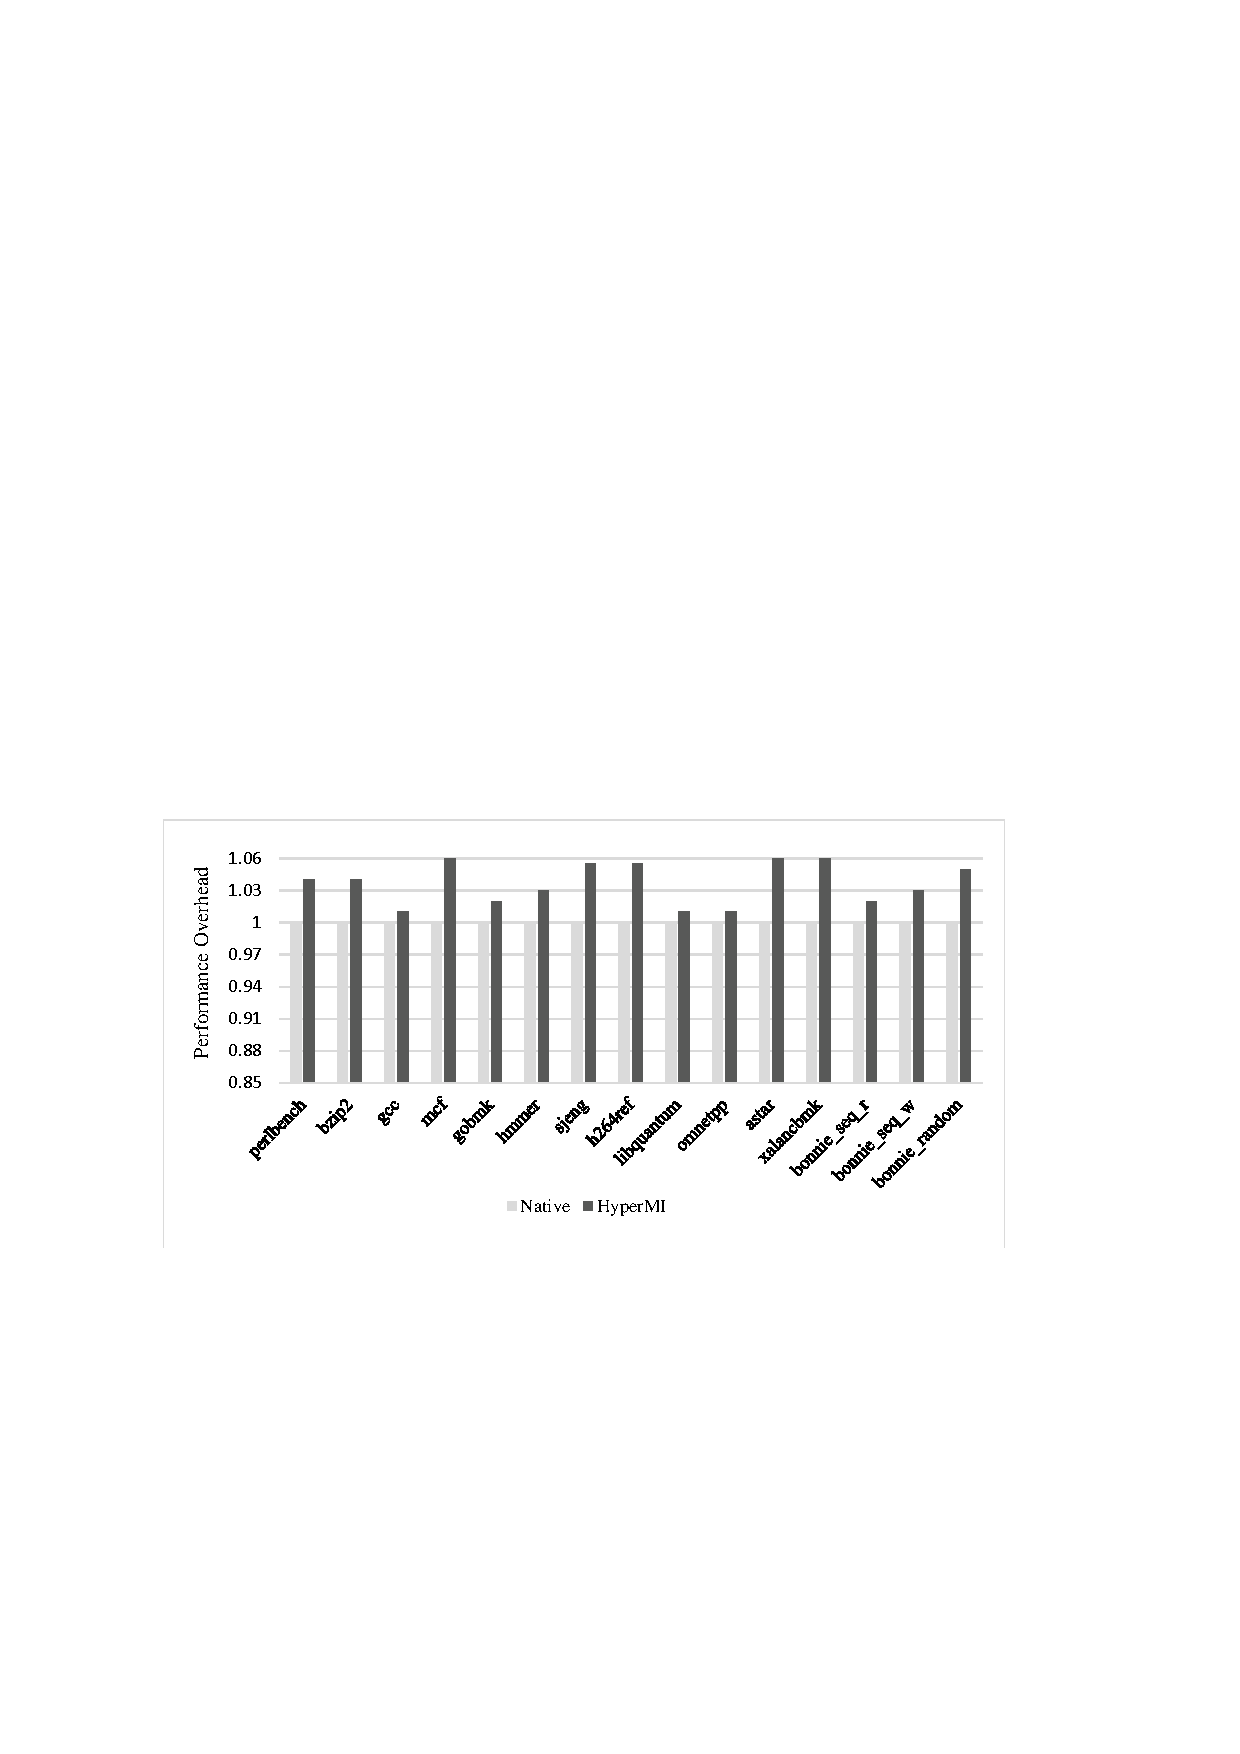
\includegraphics[width=9cm,height=5.2cm]{performance.pdf}}
\caption{Performance overhead.} \label{fig5}
\end{figure}

\subsection{Performance Evaluation}

In HyperMI, the hypervisor is modified so that HyperMI World is initialized during the boot up sequence. This includes creating a new memory page table for HyperMI, allocating memory pages, as well as creating Page-Mark table and VM-Mark table. This process introduces security verification for pages according to Page-Mark table, and security accessing for VMCS in HyperMI World during VM Exit/Entry sequence.
The kernel is modified to place hooks upon some functions.
%control registers, accessing VMCS operations, and accessing EPT operations。
% in order to achieve HyperMI World, VM Monitoring and VM Isolation.
% The contorl flow jumps to HyperMI World through the switch gate. 
introducing worlds switching overhead using switch gate.

%We do not directly compare HyperMI with previous software approaches, as they cannot support all functions simultaneously. 
In order to assess the effectiveness of all aspects of HyperMI, we conduct a set of experiments to evaluate the performance impact imposed by HyperMI against an original KVM system (the baseline). We run two groups of experiments, compare the performance overhead including benchmarks performance overhead and VM load time.
%. 
For simplicity, we only present the performance evaluation on a server with 64 cores and 32 GB memory, running at 2.0 GHz and guest VM with 2 virtual cores. The version of the hypervisor and guest VM is 3.10.1. Different experiments are based on different numbers of guest VMs with different memory size. Both the original hypervisor and HyperMI systems have the same configuration except the protection supported by HyperMI. The deviation of these experiments is insignificant. All the experiments are replicated fifty times and the average results are reported here.



\textbf{Benchmarks Performance}
%All experiments are done on a server with 64 cores and 32 GB memory, running at 2.0 GHz and 5 VMs. 
In order to obtain the impact of HyperMI on the whole system, we measure HyperMI with microbenchmarks and application benchmarks. 
We use one guest VM with 1 GB memory size. 
%All experiments are done 50 times and results are from the average.

To better understand the factor causing the performance overhead, we experiment with compute-bound benchmark (SPEC CPU2006 suite) and one I/O-bound benchmark (Bonnie++) running upon original KVM and HyperMI in a Linux VM. The experiment result described in Figure \ref{fig5}(the last three groups) shows a relatively low cost. Most of the SPEC CPU2006 benchmarks (the first twelve groups) show less than 6\% performance overhead. It's not surprising as there are few OS interactions and these tests are compute-bound. Mcf, astar, and xalancbmk with the highest performance loss allocate lots of memory. HyperMI handles Page-Mark structure and verifies the legality of page mapping when EPT updates. This can incur worlds switching which involves controlling register access and incur VM exit which involves EPT updating.
% and fewer TLB flushes with PCID technique because the two worlds are at the same privileged layer.
 For Bonnie++, we choose a 1000 MB file to perform the sequential read, write and random access. The performance loss of sequential read, write and random access is 2\%, 3\% and 5\%, not high, the main reason is that HyperMI has no extra memory operations for I/O data. The performance result shows that HyperMI introduces trivial switch overhead of two worlds and trivial overhead of memory isolation of VMs.

%{\bfseries\textbf\centering{Page-Mark Table}}
\begin{table}
\centering
\caption{execution time of vm operation(s).}\label{tabvm}
%\begin{tabular}{|c{1cm}|c|c|}
\begin{tabular}{p{2cm}|p{1.4cm}|p{1.5cm}}
\hline
{\itshape\bfseries  Test Case} & {\itshape\bfseries VM Create} & {\itshape\bfseries VM Destroy} \\
\hline
No\_HyperMI & 11.79 s &  1.75 s\\
\hline
With\_HyperMI & 12.97 s & 1.89 s\\ 
\hline
Efficiency & 1.1 & 1.08 \\
\hline
\end{tabular}
\end{table}


\textbf {VM Load Time}
% and World Switch Overhead}
The load time of a VM is a critical aspect of performance to be considered because it influences user experience. We design experiments to evaluate the performance impact of HyperMI for VM loading.
% Experiments are done with 4 VMs, each guest VM is with different memory sizes from 512MB to 4GB.
 %As expected, the VM booting time in HyperMI increases as the memory sizes increase, and the growth amplitude are more and much larger due to the world switch and page tracking caused by frequent memory allocation.
 We measure the impact of completely booting and shutdowning a VM (configured with 2 VCPU and 512MB memory). As Table \ref{tabvm} shown, the booting time is suffered a 1.1 times slowdown under HyperMI, shutdown time is suffered a 1.08 times slowdown, due to the extra overhead of worlds switching and Page-Mark table accessing in HyperMI World. Such overhead is worth for HyperMI.


\iffalse
\textbf {VM Exit/Entry Overhead}
Experiments are done on one VM with 2G memory. Network accessing can introduce lots of VM Exit, afterwards VMCS accessing in HyperMI World and world switches. In order to measure the performance impact of HyperMI, we use Netperf (version 2.7.0), a benchmark for measuring various aspects of networking performance, to determine VM Exit/Entry performance overhead. We run a netperf process in the tested VM, sending TCP or UDP streams. The performance of I/O instruction exits (i.e., VM exits triggered by the guest's I/O requests) is 2\% for TCP and 3\% for UDP, not high. 
%When we send or receive 1024-byte packets to or from an external server, HyperMI introduces xxx times VM Exit per second, xxx\% less than original KVM. 
Based on experimental results, we conclude that VMCS accessing in HyperMI World and worlds switching can be accepted.

\fi

\section{Related work}\label{sec:related}
We describe the related work from these three aspects,
% integrity verification for hypervisor,
 reconstructed hypervisor, customized hardware, and the same privilege-level isolation.
% The first aspect is considered from the perspective of protecting the hypervisor, and the other three aspects are considered from the perspective of protecting VMs.

%\subsection{Protection for Hypervisor}
\iffalse
\subsection{Integrity Verification for Hypervisor}
In order to ensure the security of the hypervisor during trusted boot and runtime, an effective and commonly used method is to verify the integrity of the hypervisor, and reduce the attack surface. For the security of the hypervisor during trusted boot, paper \cite{Petroni2007Automated} proposes control flow integrity protection policy, by verifying regularly control flow integrity behavior to detect rootkit attacks. However, attacker can detect the regular and bypass the detection. For runtime security of the hypervisor, HyperSafe \cite{Wang2010HyperSafe} and HyperCheck \cite{Wang2010HyperCheck} choose pooling-query method based on SMM to finish integrity verification of hypervisor. However, SMM doesn't support for MMU. And attackers can hide trace during polling-query intervals when comparing to event-driven monitoring.
\fi


%\subsection{Resource Isolation}

\subsection{Customized Hardware }
Some works at hardware level complete the protection of the process by extending the virtualization capabilities\cite{Moon2012Vigilare},\cite{Lee2013KI}. These tasks provide fine-grained isolation of processes and modules from the hardware level. Haven \cite{haven} uses Intel SGX\cite{Hoekstra13cuvillo,Mckeen2013Innovative} to isolate cloud services from other services and prevent cross-domain access. SGX provides fine-grained protection at the application space instead of hypervisor space, and needs developers spend time reconstructing code and dividing code into trusted part or untrusted part. SGX has requirement for version of CPU and is applied on a few platforms.% The effort \cite{Cho2016Hardware} combines the advantages of ARM TrustZone and virtualization to improve system performance, and isolate critical process components securely and efficiently.
% H-SVM\cite{Jin2015H} utilizes the hardware extension features of the CPU, and extends SMM microcode to achieve memory resource isolation among virtual machines. It deprives ability of accessing to memory resource by replacing the source code of the original hypervisor to access memory resource.
% Vigilare\cite{Moon2012Vigilare} and KI-Mon \cite{Lee2013KI} provide monitoring for access operations by introducing extra hardware. Vigilare provides a kernel integrity monitor that is architected to snoop the bus traffic of the host system from a separate independent hardware. 
% It adds extra Snooper hardware connections module to the host system for bus snooping. KI-Mon monitors write operation to system bus and handles data to write in order to check rootkit attack.
%However, for cloud providers, these approaches means high-cost and low practicality as long as they are carried out widely.
%KI-Mon monitors write operation on system bus and handles data to write in order to check rootkit attack.

\subsection{Reconstructed Hypervisor }
Except for approaches based on hardware, some works\cite{nexen,Steinberg2010NOVA,hyperlock} pay attention to software isolation. Pre-allocating physical resource and completed isolated environment for every VM can avoid VM cross-domain attack, and data leakage attack. NOVA\cite{Steinberg2010NOVA} divides hypervisor into micro-hypervisor and user hypervisor running in root mode, adopts an idea which is similar to fault domain isolation to guarantee an isolated user hypervisor for every VM. The drawback of this approach is the lack of fractional traditional hypervisor functions. HyperLock \cite{hyperlock} prepares backup KVM for every VM by copying KVM code, and ensures every VM run in own isolated space. 
%Nexen\cite{nexen} reconstructs the XEN hypervisor into one privileged security monitor, one component for shared service, backup XEN code and data for every VM, to resist attacker from exploiting known XEN vulnerabilities. 
These approaches redesign hypervisor greatly. In contrary, HyperMI adopts a feasible way to isolate VM without lots of modification of hypervisor. 

\subsection{The Same Privilege Level Isolation}
Some efforts, 
%ED-Monitor\cite{Deng2017Dancing},
 SKEE\cite{Azab2016SKEE} and SecPod\cite{Wang2015SecPod},\cite{Deng2017Dancing}, adopt the same privilege-level idea to avoid performance overhead of inter-level translation.
% ED-Monitor presents a novel approach that enables practical event-driven monitoring for compromised hypervisor in cloud computing, adopts "the same privilege level" protection against an untrusted hypervisor. The created monitor is placed at the same privilege level and in the same space with hypervisor. It relies on the mutual-protection of a
%unique pair of the techniques: Instrumentation-based Privilege Restriction (IPR) and Address Space Randomization (ASR). At the high level, IPR intercepts the most privileged operations in the Hypervisor and transfers these operations to ED-monitor, while ASR hides ED-monitor in the address space from the Hypervisor.
 %SKEE provides a lightweight secure kernel-level execution environment, it is placed at the same privilege-level with kernel. SKEE is exclusively designed for commodity ARM platforms using system characteristics of ARM. 
SKEE can only be applied to limited levels of system software in comparison with HyperMI. First, targeting ARM's 32-bit architecture, SKEE capitalizes mainly on Translation Table Base Control Register (TTBCR) for dynamic page table activation. To be more specific, SKEE creates separate page tables for the secure world and activates it in a timely manner by modifying the N field of TTBCR. However, as this hardware feature is only defined in the kernel privilege level on AArch32, SKEE is not commonly applicable to different levels of system software, such as hypervisors. %Unfortunately, SKEE faces a similar limitation on ARM's 64-bit architecture. SKEE is more focused on using the features of the ARM platform while HyperMI has no dependence on multi-platforms.
%%%%%%%The difference between HyperMI and SKEE is that HyperMI uses two sets of page tables to create the execution environment, and SKEE uses one set of page table. The design of the switch gate for HyperMI and SKEE is also different. SKEE is more focused on using the characteristic of the ARM platform while HyperMI has no dependence on multi-platforms.
%When kernel is compromised, an attacker cannot break the isolation between SKEE and the kernel, and the security of internal security tools placed at secure isolated environment is guaranteed.
SecPod, an extensible approach for virtualization-based security systems that can provide both strong isolation and the compatibility with modern hardware. The biggest difference between SecPod and HyperMI is that SecPod creates the secure isolation environment for every VM. SecPod solves the problem of VM address mapping with the assistance of shadow page table (SPT) technology.
% SecPod has two key techniques: paging delegation delegates and audits the kernel's paging operations to a secure space; execution trapping intercepts the (compromised) kernel's attempts to subvert SecPod by misusing privileged instructions.

We neither adopt software at a higher level than the hypervisor, nor use customized hardware. Inspired by the same privilege-level, we propose HyperMI World placed at the same privilege-level with hypervisor. HyperMI is independent on multi-platforms and practical for cloud providers.

\section{Conclusion}\label{sec:conclusion}
We introduce HyperMI, an approach that enables x86 platforms to support a secure isolated execution environment at the same privilege-level with hypervisor. The environment is designed to provide memory isolation protection for VMs, and event-driven runtime monitoring for interaction between hypervisor and VM. This approach, which does not rely on additional hardware devices or a higher privilege level software, has fewer changes to system and fewer requirements for types of CPU hardware device. It reflects good practicality, portability, and independence on multi-platforms. And security analysis describes protection for VM and HyperMI itself, the performance evaluation shows its efficiency by introducing negligible performance overhead. It can be implemented widely in real-world for cloud providers.

\section{Acknowledge}
We thank the anonymous reviewers fortheir valuable commens. This work is supported by the National Key R\&D Program of China (Grant N0.2016YFB0801002) and Guangdong Province Key Area R\&D Program (Grant N0.2019B010137002).

\bibliographystyle{splncs04} 
\bibliography{ref}
\end{document}
